\chapter{Annotation en rôle sémantique basée sur la connaissance}
\label{ch:srl}


Contrairement aux autres ressources pour l'annotation en rôles sémantiques, VerbNet couvre à la fois l'ensemble des verbes fréquents du vocabulaire tout en étant conçu sur des préceptes robustes le rendant utile pour les tâches de Traitement Automatique des Langues.

\section{Algorithme}

\section{Évaluation}

L'évaluation se fait sur FrameNet, ce qui permet tout simplement d'avoir une idée de la qualité de l'annotation en rôles sémantiques. Le mapping VerbNet-FrameNet maintenu par le projet SemLink est utilisé.


%\usepackage[
%    backend=biber,
%    style=authoryear-icomp,
%    ibidtracker=false,
%    doi=false,isbn=false,url=false,
%    sorting=ynt,
%    maxbibnames=99,maxcitenames=2]{biblatex}
%\addbibresource{bib/bib.bib}

Semantic role labeling has seen tremendous progress in the last
years, both for supervised and unsupervised approaches. The knowledge-based
approaches have been neglected while they have shown to bring the best results
to the related word sense disambiguation task. We contribute a simple
knowledge-based system with an easy to reproduce specification. We also present
a novel approach to handle the passive voice in the context of semantic role
labeling that reduces the error rate in F1 by 15.7\%, showing that significant
improvements can be brought while retaining the key advantages of the approach:
a simple approach which facilitates analysis of individual errors, does not
need any hand-annotated corpora and which is not domain-specific.


\section{Introduction}

Computing automatically a semantic representation of a given text has been
defined as the single greatest limitation on the general application of natural
language processing techniques \citep{dang1998investigating}. Semantic role
labeling provides such a representation where chunks of a sentence are
annotated with semantic roles that denote the sense of those chunks related to
the verb. In this work we use VerbNet \citep{kipper2006extending} and give
some details about it later. Figure~\ref{fig:example_srl} shows an example
highlighting the difficulty of the task which can not rely exclusively on
syntactic clues but also needs semantic knowledge.

\begin{figure}[ht]
    \centering
    \begin{tabular}{ccc}
        \toprule
        Carol & crushed   & the ice \\
        Agent & V         & Patient \\
        \midrule
        The ice & crushes & easily  \\
        Patient & V       &         \\
        \bottomrule
    \end{tabular}
    \caption{\label{fig:example_srl}Two annotated sentences for the carve-21.2 VerbNet class. All words are not necessarily annotated, and the position of the arguments does not directly determine the roles: the sense and voice of \textit{crush} are consistent between the two sentences but the semantic annotation differs.}
\end{figure}

Semantic role labeling has tremendously helped to compute semantic
representations and has been shown to improve multiple tasks such as
information extraction \citep{surdeanu2003using}, question-answering
\citep{shen2007using}, event extraction \citep{exner2011using},
plagarism detection \citep{osman2012improved}, machine translation
\citep{bazrafshan2013semantic} or even stock price prediction
\citep{xie2013semantic}.

Existing approaches to semantic role labeling are divided into two main
branches. The first one, supervised semantic role labeling, uses a
manually-annotated corpus and manually engineered features to train supervised
models on the task. The most used frame-semantics resource and associated
annotated corpus in this domain is FrameNet \citep{baker1998berkeley}.
While this approach yields the best performance \citep{das2013frame}, the
cost is high: the corpus used are annotated over several years and it would be
in general too long and costly to annotate a new corpus for each new considered
domain. To address those issues, the second mainstream approach, named semantic
role induction, uses fully unsupervised methods: given a corpus, the goal is to
cluster all verbs sharing the same behavior. While this is completely general,
the results are noisier and the semantic roles are only induced and cannot
always be mapped to human-understandable labels such as \textit{Agent} or
\textit{Topic}.

A third approach, knowledge-based semantic role labeling
\citep{swier2004unsupervised,swier2005exploiting}, has not received much
attention lately. The goal is to use external lexical-semantic resources for
each new considered language and to use those resources to annotate text. The
quality of annotation suffers, but bringing semantic role labeling to new
domains and languages becomes easier: no corpus has to be hand-annotated.

Existing work on the knowledge-based semantic role labeling task is now dated
but the resources have much improved since then:
\citep{swier2005exploiting} could only use VerbNet 1.5, but VerbNet 3.2 is
now available. They also had to use a custom mapping to FrameNet for the evaluation 
of their method while the SemLink project has provided us an ``official'' 
FrameNet-VerbNet mapping. FrameNet has been also vastly
improved and extended since 2005: new training data is available, many
corrections have been made, and a full-text corpus can now be used to evaluate
semantic role labeling in a more realistic way.

While the present work\footnote{This work was partially funded by the ANR
ASFALDA ANR-12-CORD-0023 project.} is similar to
\citep{swier2005exploiting}, we do believe that there is an opportunity to
reevaluate knowledge-based semantic role labeling, precisely because the last
work we are aware of dates from 2005 and is difficult to reproduce. We indeed
show that incorporating passive voice detection to the task improve results by
15.7\%: improvements are still possible.

\section{Knowledge-based semantic role labeling}
\label{sec:srl}

Knowledge-based semantic role labeling refers to algorithms that don't use a
priori training data which would be biased and hamper performance on new
domains. The "knowledge" is contained in VerbNet-like databases which encode
syntactic and semantic informations about verbs in a way that allows one to map
syntactic structure to semantic roles. Previous work on this task used the word
"unsupervised" instead of "knowledge-based", but unsupervised semantic role
labeling now refers to truly unsupervised work where no semantic knowledge is
needed at all.

In this work, we use the English VerbNet \citep{kipper2006extending}, a
freely available hierarchical verb lexicon based on Levin classes
\citep{levin1993english} which encodes into \emph{frames} the mapping
between diathesis alternations and semantic roles assigned to syntactic chunks.
For a given frame, VerbNet can map between NP V NP and Agent V Theme: this
means that in this situation the first noun phrase should be mapped to the
Agent role while the second one should be mapped the Theme role. Our goal is to
use this mapping information to transform syntactically-analyzed sentences into
semantically-analyzed sentences. The mapping can be unambiguous when only one
VerbNet frame matches a given dependency graph. In other cases, different options are
possible. This occurs when: 

\begin{itemize}

    \item a predicate is present in multiple VerbNet classes which share the same
    diathesis alternations but do not map to the same roles.

    \item syntax-semantics mappings are ambiguous and do not fully determine the
    semantic role that should be used.

\end{itemize}

Without annotated data, those ambiguities cannot be resolved. However, once an
initial mapping is done, it becomes possible to use those in-domain mapping to
learn simple probabilistic models which will allow to label new verbs and their
roles with high precision.

% GC The sentence below comes strangely at this place but I don't find how to 
% rewrite or move it right now.
Our error analysis in the evaluation section shows that important error 
reductions can be achieved while
staying in the framework of knowledge-based semantic role labeling, reaffirming
this approach as useful and promising again. We now describe in details the 
various steps of our algorithm.

\subsection{Argument identification}

This first step identifies syntactic chunks that will bear semantic roles in the two
future stages.  This standard step in semantic role labeling analyses a
sentence syntactically or splits it into chunks and chooses syntactic trees as
arguments.  We use \citep{lang2011unsupervised} eight rules to select
nodes that are likely to have semantic roles. This step selects too much
candidates, but they are filtered out by the subsequent steps.
% GC FUTURE Examples

\subsection{Frame matching}

This step matches role fillers to roles when it is possible to do so in an
unambiguous way. It merges in one step what is traditionally done in two steps:
frame identification and actual role labeling. We first map our arguments to a
VerbNet-style construction where the arguments are ordered and the first one
appears before the verb. Those positions determine the "grammatical function"
(or slot): the first argument is a syntactic subject, the second one is an
object, the third one is an indirect object, and chunks whose head word is a
preposition are "prepositional objects".

Once the grammatical functions have been assigned, we match all possible
VerbNet frames given the predicate. For example, the \textit{classify}
predicate exists in two VerbNet frames: \textit{characterize-29.2} and
\textit{classify-29.10}. The possible frames are:

\begin{itemize}
    \item NP.Agent V NP.Theme (as) S\_ING.Attribute
    \item NP.Agent V NP.Theme to be ADJ.Attribute
    \item NP.Agent V NP.Theme as PP.Attribute
    \item NP.Agent V NP.Theme
    \item NP.Agent V NP.Theme as PP.Goal
    \item NP.Agent V NP.Theme in PP.Location
\end{itemize}

Given the sentence \emph{The company also classifies short and wide radius
ruts according to their severity} which is of the form NP V NP according PP, we
only know how to match the first two noun phrases (Agent, then Theme). There is
no possible matching for the third argument: there cannot be one, VerbNet
doesn't encode that \emph{according} is a possible preposition contrary as \emph{in}
and \emph{as}. VerbNet authors are currently working on the issue of adding new
information based on syntactic and collocational information drawn from very
large corpora \citep{bonial2013expanding}.

\subsection{Probability models}

Now that a part of the corpus has been annotated, we can use this information
to annotate new ambiguous role fillers. This is still unsupervised as we only
use data extracted by our own system for the text we need to annotate. Role
fillers are ambiguous when two or more roles are possible. Several probability
models are considered which assign probabilities: the best role filler is then
chosen.

\paragraph{predicate-slot}

The predicate-slot model uses two informations to determine the role of a given
role filler: the predicate used, and the detected grammatical function.  For
example, the Direct Object of the verb ``neglect'' will always be "Theme" based
on existing data. While the precision is high, it only assigns roles to 40\% of
arguments: for the other 60\%, we don't have any information on this specific
(predicate, grammatical function) pair.

\paragraph{slot}

The slot model does not use the predicate information which is sometimes too
sparse. It simply assigns roles based on grammatical functions. In addition to
the grammatical functions, the preposition can also be used to assign roles to
role fillers. For example, the preposition \textit{of} maps to Attribute, Theme
and Topic (in this order) in our FrameNet corpus. When faced with an ambiguous
mapping, this means this probability model will choose the first role that
matches with the possible semantic roles.

Those two simple probabilistic models are complementary: one has a high
precision but does not cover unseen verbs, while the other one helps to assign
roles to every verb. However, we chose to not use the second one in its current form due to its low
precision.

\section{Passive voice handling}

Error analysis revealed that passive voice was a common source of errors in our
corpus. Indeed, VerbNet does not encode the passive voice since it is a
syntactic phenomenon: it is up to the syntactic analyser to recognize that the
real subject is not where we expect it to be. Most syntactic analysers do not
handle deep structure. Handling such structures can be seen as an intermediate
step between syntactic analysis and semantic role labeling
\citep{bonfante2011modular,ribeyre2013systeme}.

We handled passive voice in the context of VerbNet by transforming VerbNet
syntactic frames temporarily whenever a passive voice is detected, that is
verbs in the past participle form which are governed by a form of the verb ``to
be''. Given a VerbNet frame such as \textit{NP.Agent V NP.Recipient NP.Theme},
we produce two transformations:

\begin{itemize}
    \item NP.Recipient V NP.Theme
    \item NP.Recipient V NP.Theme by NP.Agent
\end{itemize}

Now that the transformation is done, when faced with passive uses of verbs, we
simple use the new frames instead of the original ones to perform the mapping.
This gives better result as passive voices were always wrongly identified
(Table~\ref{table:results}).

\section{Evaluation}

Evaluation is currently performed against FrameNet which is one of the standard
resource for semantic role labeling. The full-text corpus is balanced,
featuring texts from multiple sources: the Wall Street Journal, the AQUAINT and
MASC corpora, and other miscellaneous texts.

\subsection{Corpora and tools}

In this experiment, we are using the full-text corpus of FrameNet 1.5, VerbNet
3.2, the VerbNet-FrameNet role mapping version
1.2.2c\footnote{\url{http://verbs.colorado.edu/semlink/1.2.2c/vn-fn/}}. Only
core arguments are considered since VerbNet often ignores the non-core FrameNet
arguments.

When working on the full semantic-parsing task, we use MST parser 0.5.0
\citep{mcdonald2006multilingual}. The parser is trained on a modified Wall
Street Journal corpus modified using NP
bracketing\footnote{\url{http://sydney.edu.au/engineering/it/~dvadas1/}} and
the LTH conversion tool for CONLL
conversion\footnote{\url{http://nlp.cs.lth.se/software/treebank_converter/}}.
Since FrameNet uses parts of the Wall Street Journal corpus, we removed six
files before training: 0558, 0089, 0456, 1778, 1286 and 1695. This ensures the
MST parser never has to parse sentences from the training set and avoids bias.
The FrameNet part-of-speech tags were converted from the BNC tagset to the WSJ
tagset using manually-defined rules (Table~\ref{table:tagset_rules}). On the
six files mentioned earlier, this reduces the number of part-of-speech tags
differences from 23\% to 3\%.

\begin{table}[hb]
    \centering
    \begin{tabular}{ccc|ccc}
        \toprule
        JJ   &$\to$& ADJ    & JJR  &$\to$& NP     \\
        JJS  &$\to$& NP     & MD   &$\to$& S      \\
        NN   &$\to$& NP     & NNP  &$\to$& NP     \\
        NNPS &$\to$& NP     & NNS  &$\to$& NP     \\
        NP   &$\to$& NP     & NPS  &$\to$& NP     \\
        PP   &$\to$& PP     & PRP  &$\to$& NP     \\  
        RB   &$\to$& ADV    & TO   &$\to$& to S   \\
        VB   &$\to$& S      & VBD  &$\to$& S      \\
        VBG  &$\to$& S\_ING & VBN  &$\to$& ADJ    \\
        VBP  &$\to$& S      & VBZ  &$\to$& S      \\
        WDT  &$\to$& NP     & \$   &$\to$& NP     \\  
        CD   &$\to$& NP     & DT   &$\to$& NP     \\
        \bottomrule
    \end{tabular}
    \caption{\protect\centering\label{table:tagset_rules}BNC to WSJ conversion rules}
\end{table}

% FUTURE SEMAFOR MXPOST/MST

\subsection{Evaluation procedure}

\begin{table*}[t!]
    \centering
    \begin{tabular}{lcccc}
        \toprule
        Task                                           & F1        & Accuracy \\
        \midrule
        FM                                             & 70.48\%   & 53.09\%  \\
        FM + predicate-slot (gold args)                & 72.02\%   & 58.28\%  \\
        FM + passive + predicate-slot (gold args)      & 76.40\%   & 62.72\%  \\
        \midrule
        Identification + FM                            & 46.75\%   & 29.12\%  \\
        Identification + FM + predicate-slot           & 46.78\%   & 33.49\%  \\
        \bottomrule
    \end{tabular}
    \caption{\protect\centering\label{table:results}Results on different tasks. FM is frame matching. Lines with \emph{passive} include the passsive voice detection. Identification is argument identification.}
\end{table*}

We feed each FrameNet sentence in the corpus to our system which performs
semantic role labeling (section \ref{sec:srl}). For each role filler annotated
in the FrameNet corpus with a verbal predicate, we use the mapping to know what
is the set of possible VerbNet roles given the FrameNet frame. This is possibly
ambiguous, mostly because a FrameNet frame can refer to multiple VerbNet
classes: we don't evaluate against those roles.

Another difficulty is that the mapping isn't complete: some VerbNet classes
cannot be mapped from FrameNet to VerbNet. Indeed, only 4605 out of 10052 roles
are mapped: we only evaluate against those frames.

We measure precision, recall, and accuracy of correct role/role filler
associations out of the FrameNet ones that have been converted to VerbNet-style
roles. 10\% of the corpus was used as a test set, while the other 90\% were
manually scanned to check for issues in our algorithm.

Table~\ref{table:results} shows results on different tasks. The first three
tasks are evaluated on gold arguments: argument identification was not needed, which
definitely helps the models. The following two tasks are evaluated on the full
frame-semantic parsing task: arguments are identified automatically based on
automatic parses. The full model is "Identification + FM + predicate-slot": it
associates argument identification, frame matching and the predicate-slot
probabilistic model.

The main takeaway is that argument identification needs to be improved
significantly to help our model reach acceptable levels of performance. The
first issue is that only around 76\% of arguments are present in our dependency
parses. The second issue is the heuristics we used for argument identification:
they need to be analysed more thoroughly or replaced with alternatives
approaches \citep{abend2009unsupervised}.

\begin{table}[ht]
    \centering
    \begin{tabular}{lccc}
        \toprule
        Model          & Precision & Coverage \\
        \midrule
        slot           & 52.45\% & 100\% \\
        predicate-slot & 68.33\% & 38.33\% \\
        \bottomrule
    \end{tabular}
    \caption{\protect\centering\label{table:probabilisticresults}Results for probabilistic models}
\end{table}

Table~\ref{table:probabilisticresults} highlights the complementary nature of
our models: the predicate slot model has better precision but lower coverage
than the slot model.

\begin{figure}[t]
    \centering
    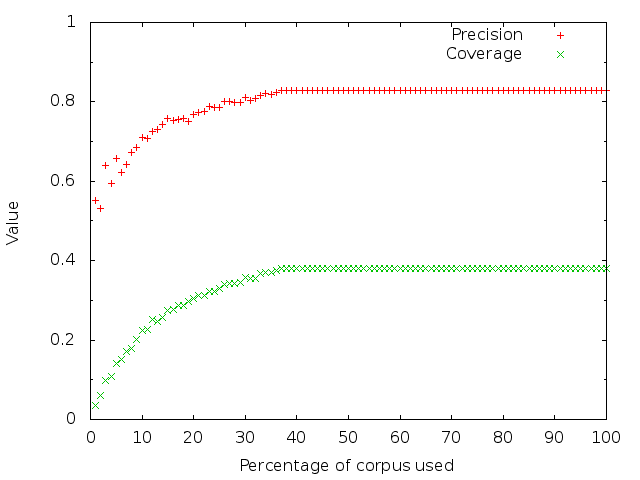
\includegraphics[width=0.45\textwidth]{fig/slot-predicate-percents.png}
    \caption{\label{fig:slot_predicate} slot-predicate model performance when training over a part of the training corpus: from 0 to 100\%.}
\end{figure}

Figure~\ref{fig:slot_predicate} highlights that we don't need the whole corpus
to attain this level of performance. This is interesting because our methods
can operate efficiently on a small domain-specific corpus and because the full
potential of this corpus is not fully realized.

\subsection{SEMAFOR comparison}

SEMAFOR \citep{das2013frame} is currently the state-of-the-art supervised
frame-semantic parser on the SemEval test sets and FrameNet full-text corpus.
It annotates all FrameNet parts-of-speech while we only concentrate on verbs.
It achieves 46.49\% F1 score on the full task, which should be compared with
the 25\% F1 score of our system.  SEMAFOR uses three stages for semantic
parsing:

\begin{itemize}
    \item target identification
    \item frame identification
    \item argument identification
\end{itemize}

As such, it cannot be compared directly with our system which does not solve
the task using the same structure. However, it is interesting to note how
important is the training data: for frame identification with gold
targets\footnote{Results for automatic targets were only given for the SemEval
2007 dataset}, the same models grows from 74.21\% to 90.51\% in F1-score for
frame identification when switching from the SemEval 2007 dataset to the
FrameNet 1.5 dataset. Likewise, for argument identification and gold
frames\footnotemark[\value{footnote}], the results grow from 48.09\% to
68.93\%. The size of the training data is extremely important, while our
approach is better suited to domain adaptation where large annotated corpora
are seldom available.

\section{Future work}

Future includes evaluating our approach on domain-specific corpora such as the
Kicktionary \citep{schmidt2009kicktionary}, the Robocup dataset
\citep{chen2008learning} or the Situated Language dataset
\citep{bordes2010towards} and compare our method with existing
domain-specific semantic role labeling work
\citep{wyner2010lexical,hadouche2011annotation,goldwasser2013leveraging}.

We also plan to incorporate more domain-specific information such as semantic
similarity between existing role fillers to detect roles that are placed in an
unusual way.

Finally, in the same way that handling the passive voice produced better
results, we plan to integrate deep structure handling to our system. A common
case of errors is coordination. When two verbs share the same subject, the
syntactic analysis should properly link from each verb to the subject. Here are
two examples: first with the verbs blunder and, then with the verbs steal and
share:

\begin{itemize}
    \item You are not fair when you belittle Sheik Bin Baz 's blunder and
          exaggerate the one by Sheik Maqdasi ...
    \item Hostile and even friendly nations routinely steal information from
          U.S. companies and share it with their own companies
\end{itemize}

More specifically, we currently plan to integrate the system from
\citep{ribeyre2013systeme} as it handles complex deep structure situations
by adding simple rules to the system to take into account new syntactic
constructions, and will allow to handle all considered deep structure links in
a cohesive way.

\section{Conclusion}

We have implemented a knowledge-based semantic role labeling system. We used
publicly available versions of data and tools which make our work easily
reproducible, now and in the future. We have started to improve the basic
algorithm with enhancements that improve its results. The current results are
probably still insufficient to improve the results of natural language
processing applications such as information retrieval or text summarization,
but the foreseeable improvements make the approach promising. The independence
of the approach with respect to annotated corpus makes it interesting even if
raw performance is as expected lower than the one of supervised approaches.
Besides the future work above, our forthcoming introduction of corpus-based
syntactico-semantic selectional restrictions is a next step.
